\section{Marco teórico}
\subsection{Historia de los códigos éticos en investigación}
\begin{frame}{Historia de los códigos éticos en investigación}
    \begin{minipage}{0.45\linewidth}
    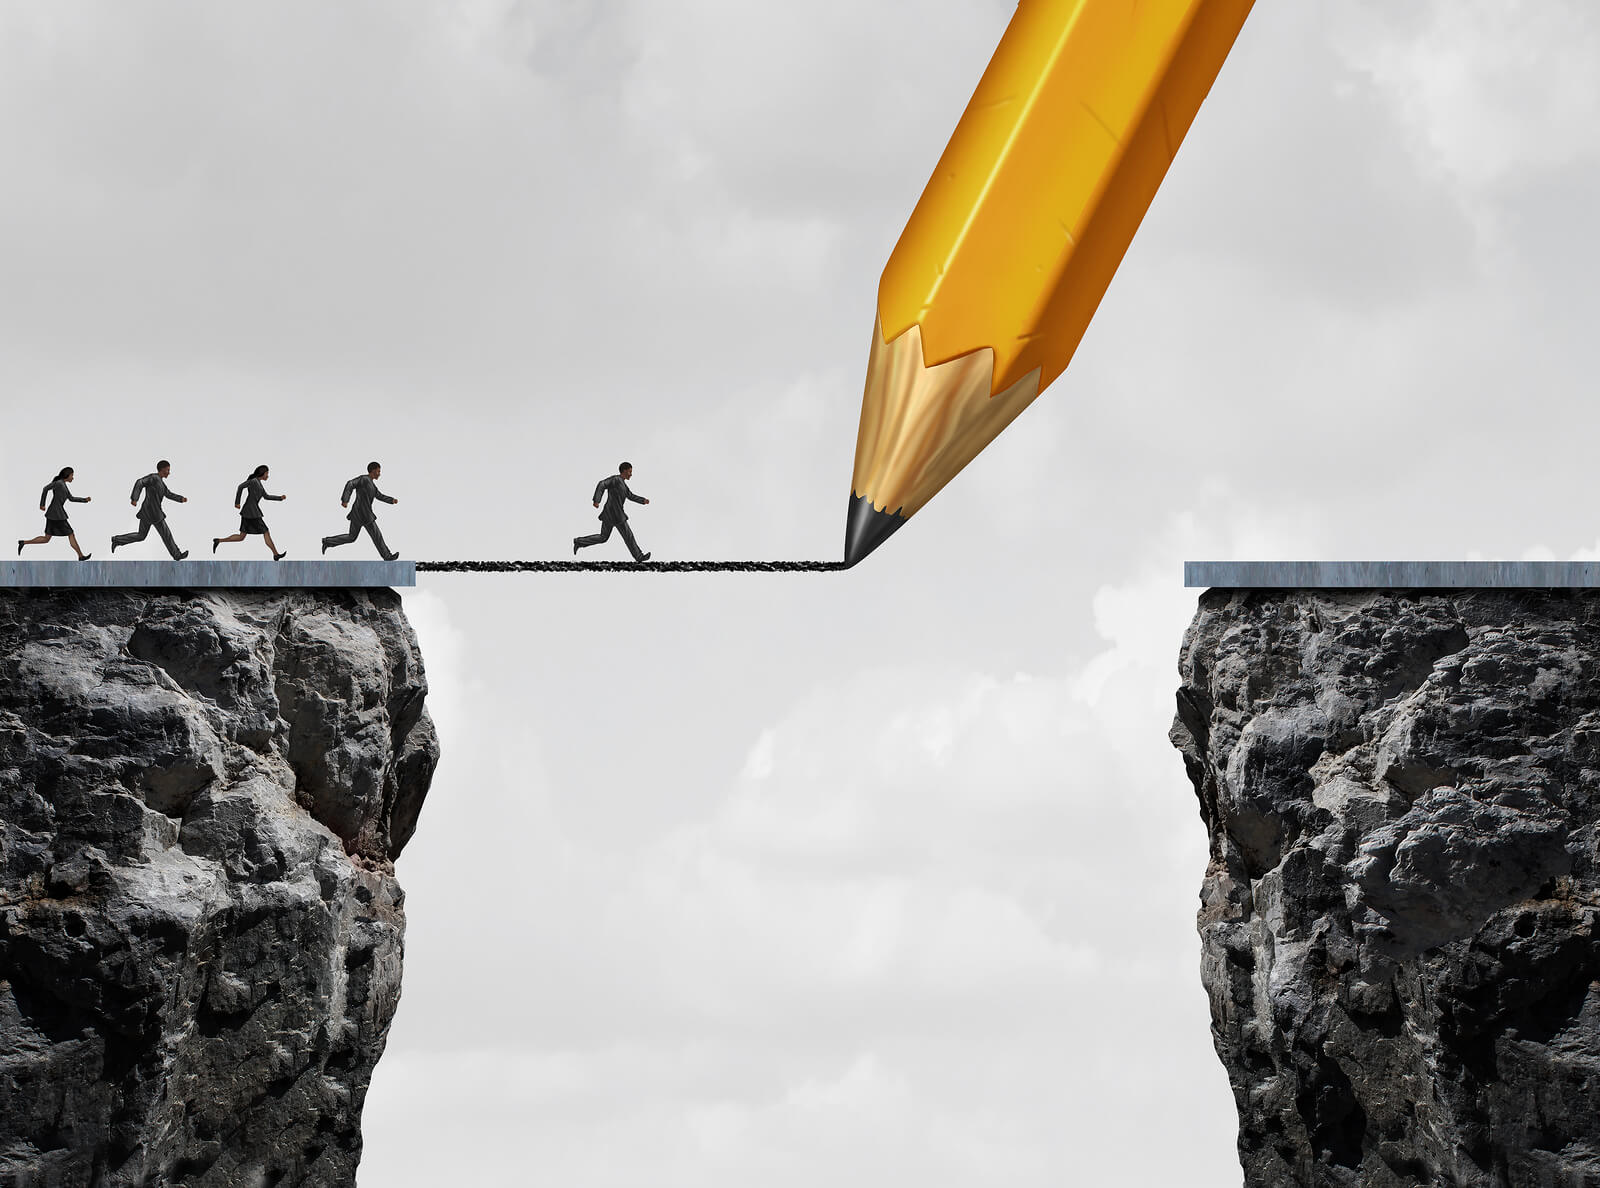
\includegraphics[scale=0.1]{images/ima4.jpg}
    \end{minipage}
    \begin{minipage}{0.5\linewidth}
    Las circunstancias históricas y los valores de los tiempos influyeron directamente en la creación y evolución
    de los códigos éticos en la investigación científica, siendo su desarrollo acelerado pr múltiples situaciones partículares,
    tanto en sus procesos como en las disciplinas de conocimiento vinculadas en su creación.
\end{minipage}
\end{frame}
\begin{frame}{Historia de los códigos éticos en investigación}
    \begin{minipage}{0.5\linewidth}
        McNeil en su documento destaca 
        que en el año 1900 Alemania fue el primer país que generó un código ético para su uso local, siendo esta normativa remitida
        a los directores de las clínicas hospitalitarias con el fin de limitar los experimentos médicos y obligando a los especialistas 
        a describir sus intervenciones sanitarias a los adultos competentes.
    \end{minipage}
    \begin{minipage}{0.45\linewidth}
        \centering
        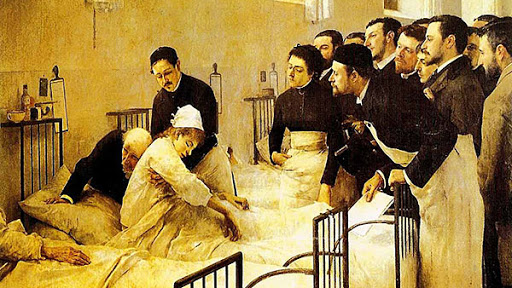
\includegraphics[scale=0.4]{images/ima5.jpg}
    \end{minipage}
\end{frame}
\begin{frame}{Historia de los códigos éticos en investigación}
        Al momento de haber establecido códigos de ética en la investigación con seres humanos se produjo en gran medida, por las revelaciones de 
        los experimentos médidos llevados a cabo por médicos nazis en los campos de concenrtración alemanes durante el Tercer Reich. \\
        \centering
        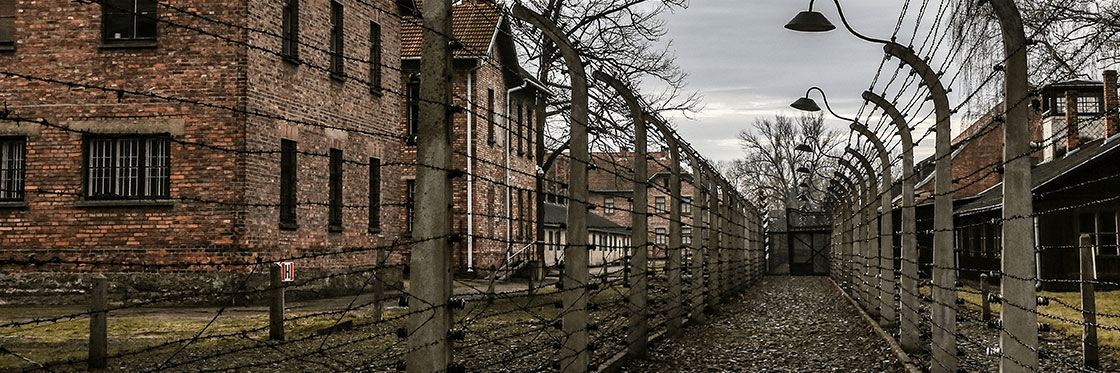
\includegraphics[scale=0.27]{images/ima6.png}
\end{frame}
\begin{frame}{Historia de los códigos éticos en investigación}
    \begin{minipage}{0.5\linewidth}
        \centering
        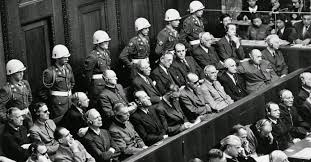
\includegraphics[scale=0.65]{images/ima7.jpeg}
    \end{minipage}
    \hspace{0.3cm}
    \begin{minipage}{0.45\linewidth}
    A partir de 1945 se realizaron esfuerzos claves para plantear los principios éticos en la investigación científica a nivel mundial. En 1947, el desarrollo
    del \textit{Código de Nuremberg}, el cual orienta con principios considerados fundamentales para el establecimiento de procesos de investigación
    con seres humanos,
    \end{minipage}
\end{frame}
\subsection{Código de buenas prácticas}
\begin{frame}{Código de buenas prácticas}
    \begin{minipage}{0.5\linewidth}
    En la comunidad científica internacional se dispone, actualmente, de un amplio consenso
    con respecto a los componentes más importantes de todo aquello que constituyen unas
    buenas prácticas científicas. Las dos finalidades principales de las BPC son la mejora
    de la calidad de la ciencia y la prevención de problemas de integridad de la investigación.
\end{minipage}
\hspace{0.2cm}
\begin{minipage}{0.45\linewidth}
    \centering
    
\includegraphics[scale=0.4]{images/ima8.jpg}
\end{minipage}
\end{frame}
\section{Difusión de resultados de la investigación}
\subsection{Autoría}
\begin{frame}{Difusón de resultados - Autoría}
    Para poder tener la condición plena de autor de un trabajo publicado será necesario cumplir con todas las condiciones siguientes:
\begin{enumerate}
    \item Que exista una contribución sustancial a la concepción o diseño del trabajo o a la adquisición,
    análisis o a la interpretación de los datos.
    \item Que se haya participado en la redacción del trabajo o en la revisión crítica de su contenido
    intelectual.
    \item Que se haya intervenido en la aprobación de la versión final que vaya a ser publicada.
    \item Que se tenga capacidad de responder de todos los aspectos del artículo de cara a asegurar
    que las cuestiones relacionadas con la exactitud o integridad de cualquier parte del trabajo
    están adecuadamente investigadas y resueltas.
\end{enumerate}
\end{frame}
\begin{frame}{Difusón de resultados - Autoría}
    \begin{itemize}
        \item El primer coautor es la persona que ha hecho la contribución más importante en la
        investigación y ha preparado el primer borrador del artículo
        \item El último autor es la persona que dirige la investigación o que tiene la última
        responsabilidad en el protocolo de investigación.
        \item El resto de coautores pueden aparecer ordenados por orden de contribución y, en
        algunos casos, si la contribución de todos ellos es similar, por orden alfabético, con
        mención expresa de ello.
    \end{itemize}
\end{frame}
\begin{frame}{Difusón de resultados - Publicación}
    \begin{minipage}{0.45\linewidth}
        \centering
        
\includegraphics[scale=0.2]{images/ima9.jpg}
    \end{minipage}
    \hspace{0.3cm}
    \begin{minipage}{0.5\linewidth}
    La difusión de los resultados es un deber ético de los investigadores, como contribución al incremento
y al avance del conocimiento, una parte escencial del proceso es la redención de cuentas de la utilización 
de los medios públicos para la investigación.
    \end{minipage}
\end{frame}
\section{Evaluación y revisión}
\begin{frame}{Evaluación y revisión}
        Las revisiones, en todas sus facetas (envíos para publicación, ascensos laborales, financiación de
proyectos, nombramientos de plazas) deben estar suficientemente razonadas y ser claras, precisas
e imparciales.\vspace{0.7cm}\\
\centering
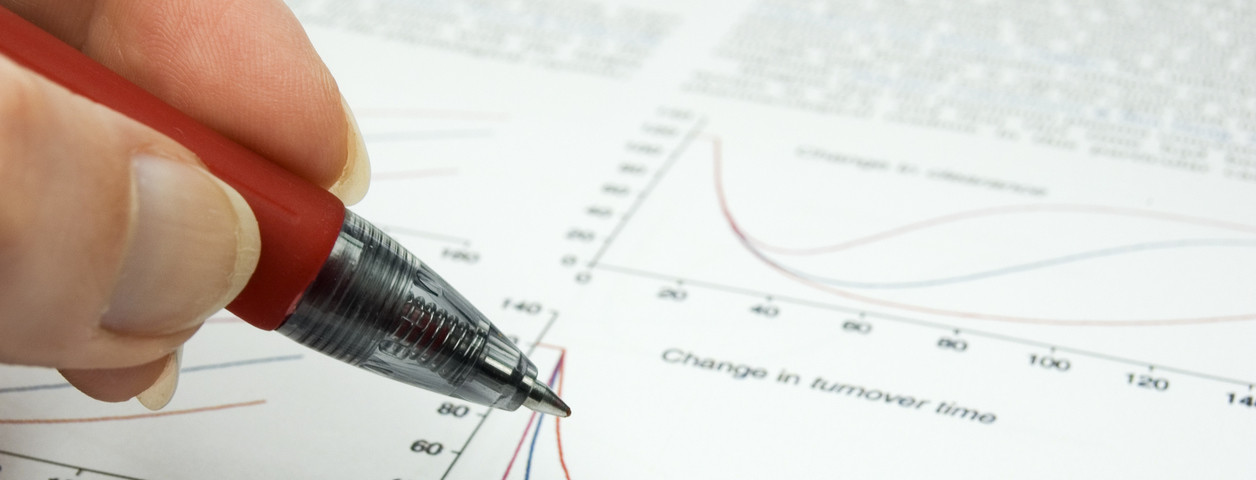
\includegraphics[scale=0.7]{images/ima10.jpg}
\end{frame}
\section{Violaciones de la integridad de la investigación}
\begin{frame}{Violaciones de la integridad de la investigación}
    \begin{minipage}{0.7\linewidth}
        La mala conducta en investigación científica consiste en el incumplimiento de las buenas prácticas
científicas por parte de los investigadores, ya sea de manera intencional o por negligencia causando 
una lesión al proceso de la investigación,  degradando las relaciones entre los investigadores, sobre explotando de la confianza
y credibilidad de la investigación exponiendo así a las personas participantes en la investigación, a la sociedad en su conjunto y al medio 
ambiente en daños innecesarios.
    \end{minipage}
    \begin{minipage}{0.25\linewidth}
        \centering
        
\includegraphics[scale=0.35]{images/ima11.jpg}
    \end{minipage}
\end{frame}
\subsection{Mala conducta y otras prácticas inaceptables en la investigación}
\begin{frame}{Mala conducta y otras prácticas inaceptables en la investigación}
    \begin{itemize}
        \item La fabricación, que consiste en la invención de los resultados y en su registro como si fueran
        reales.
        \item La falsificación, que consiste en la manipulación de los materiales, del equipamiento o del proceso
        de investigación o la modificación, omisión o supresión de datos o resultados sin justificación.
        \item El plagio, que consiste en el uso de las ideas o el trabajo de otras personas sin otorgar el crédito
        suficiente a las fuentes originales, con la consiguiente violación de los derechos de los autores
        originales a su producto intelectual.
    \end{itemize}
\end{frame}
\begin{frame}{Mala conducta y otras prácticas inaceptables en la investigación}
    \begin{itemize}
        \item Adulterar la autoría de un trabajo y minusvalorar o no reconocer el papel de otros investigadores
        en las publicaciones.
        \item Incurrir en el autoplagio, incluyendo las traducciones a otros idiomas, sin el reconocimiento
        debido o sin citar apropiadamente los trabajos originales.
        \item Citar selectivamente determinadas referencias con objeto de resaltar los hallazgos propios o de
        complacer a los directores de las revistas, a los revisores o a los colegas.
        \item Retrasar o dificultar indebidamente el trabajo de otros investigadores.
        \item Utilizar la posición de autoridad para fomentar violaciones de la integridad científica.
    \end{itemize}
\end{frame}
\section{Ejemplos de malas conductas en la investigación}
\begin{frame}{Ejemplos de malas conductas en la investigación}
    \changefontsizes{10pt}
    \begin{itemize}
        \item Caso reportado en \textit{Research Ethics: A Philosophical Guide to the Responsible Conduct of Research}\\
        En este documento se indicaron que la conducta no ética más frecuente es la falsificación de datos de la investigación.
        \textit{Los coordinadores de los posgrados de Astrofísica y de Ciencias Matemáticas expresaron
        que hay investigadores que anuncian sus resultados con base en hechos falsos y que una de las
        causas es la enorme presión por publicar.}
        \item Caso reportado en \textit{El papel de la ética en la investigación científıca y educación superior.}\\
        Presentan un \textit{abuso de los apoyos financieros del
        erario público por parte del estudiante durante sus estudios de posgrado}, indicando que \textit{
            cuando un estudiante acepta una beca lo hace con el compromiso de dedicar tiempo completo a sus
    estudios, y se estaría incurriendo en una conducta éticamente cuestionable si esta premisa no
    se cumple}
    \end{itemize}
\end{frame}